\documentclass[1p]{elsarticle_modified}
%\bibliographystyle{elsarticle-num}

%\usepackage[colorlinks]{hyperref}
%\usepackage{abbrmath_seonhwa} %\Abb, \Ascr, \Acal ,\Abf, \Afrak
\usepackage{amsfonts}
\usepackage{amssymb}
\usepackage{amsmath}
\usepackage{amsthm}
\usepackage{scalefnt}
\usepackage{amsbsy}
\usepackage{kotex}
\usepackage{caption}
\usepackage{subfig}
\usepackage{color}
\usepackage{graphicx}
\usepackage{xcolor} %% white, black, red, green, blue, cyan, magenta, yellow
\usepackage{float}
\usepackage{setspace}
\usepackage{hyperref}

\usepackage{tikz}
\usetikzlibrary{arrows}

\usepackage{multirow}
\usepackage{array} % fixed length table
\usepackage{hhline}

%%%%%%%%%%%%%%%%%%%%%
\makeatletter
\renewcommand*\env@matrix[1][\arraystretch]{%
	\edef\arraystretch{#1}%
	\hskip -\arraycolsep
	\let\@ifnextchar\new@ifnextchar
	\array{*\c@MaxMatrixCols c}}
\makeatother %https://tex.stackexchange.com/questions/14071/how-can-i-increase-the-line-spacing-in-a-matrix
%%%%%%%%%%%%%%%

\usepackage[normalem]{ulem}

\newcommand{\msout}[1]{\ifmmode\text{\sout{\ensuremath{#1}}}\else\sout{#1}\fi}
%SOURCE: \msout is \stkout macro in https://tex.stackexchange.com/questions/20609/strikeout-in-math-mode

\newcommand{\cancel}[1]{
	\ifmmode
	{\color{red}\msout{#1}}
	\else
	{\color{red}\sout{#1}}
	\fi
}

\newcommand{\add}[1]{
	{\color{blue}\uwave{#1}}
}

\newcommand{\replace}[2]{
	\ifmmode
	{\color{red}\msout{#1}}{\color{blue}\uwave{#2}}
	\else
	{\color{red}\sout{#1}}{\color{blue}\uwave{#2}}
	\fi
}

\newcommand{\Sol}{\mathcal{S}} %segment
\newcommand{\D}{D} %diagram
\newcommand{\A}{\mathcal{A}} %arc


%%%%%%%%%%%%%%%%%%%%%%%%%%%%%5 test

\def\sl{\operatorname{\textup{SL}}(2,\Cbb)}
\def\psl{\operatorname{\textup{PSL}}(2,\Cbb)}
\def\quan{\mkern 1mu \triangleright \mkern 1mu}

\theoremstyle{definition}
\newtheorem{thm}{Theorem}[section]
\newtheorem{prop}[thm]{Proposition}
\newtheorem{lem}[thm]{Lemma}
\newtheorem{ques}[thm]{Question}
\newtheorem{cor}[thm]{Corollary}
\newtheorem{defn}[thm]{Definition}
\newtheorem{exam}[thm]{Example}
\newtheorem{rmk}[thm]{Remark}
\newtheorem{alg}[thm]{Algorithm}

\newcommand{\I}{\sqrt{-1}}
\begin{document}

%\begin{frontmatter}
%
%\title{Boundary parabolic representations of knots up to 8 crossings}
%
%%% Group authors per affiliation:
%\author{Yunhi Cho} 
%\address{Department of Mathematics, University of Seoul, Seoul, Korea}
%\ead{yhcho@uos.ac.kr}
%
%
%\author{Seonhwa Kim} %\fnref{s_kim}}
%\address{Center for Geometry and Physics, Institute for Basic Science, Pohang, 37673, Korea}
%\ead{ryeona17@ibs.re.kr}
%
%\author{Hyuk Kim}
%\address{Department of Mathematical Sciences, Seoul National University, Seoul 08826, Korea}
%\ead{hyukkim@snu.ac.kr}
%
%\author{Seokbeom Yoon}
%\address{Department of Mathematical Sciences, Seoul National University, Seoul, 08826,  Korea}
%\ead{sbyoon15@snu.ac.kr}
%
%\begin{abstract}
%We find all boundary parabolic representation of knots up to 8 crossings.
%
%\end{abstract}
%\begin{keyword}
%    \MSC[2010] 57M25 
%\end{keyword}
%
%\end{frontmatter}

%\linenumbers
%\tableofcontents
%
\newcommand\colored[1]{\textcolor{white}{\rule[-0.35ex]{0.8em}{1.4ex}}\kern-0.8em\color{red} #1}%
%\newcommand\colored[1]{\textcolor{white}{ #1}\kern-2.17ex	\textcolor{white}{ #1}\kern-1.81ex	\textcolor{white}{ #1}\kern-2.15ex\color{red}#1	}

{\Large $\underline{12a_{1171}~(K12a_{1171})}$}

\setlength{\tabcolsep}{10pt}
\renewcommand{\arraystretch}{1.6}
\vspace{1cm}\begin{tabular}{m{100pt}>{\centering\arraybackslash}m{274pt}}
\multirow{5}{120pt}{
	\centering
	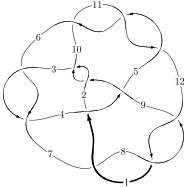
\includegraphics[width=112pt]{../../../GIT/diagram.site/Diagrams/png/1972_12a_1171.png}\\
\ \ \ A knot diagram\footnotemark}&
\allowdisplaybreaks
\textbf{Linearized knot diagam} \\
\cline{2-2}
 &
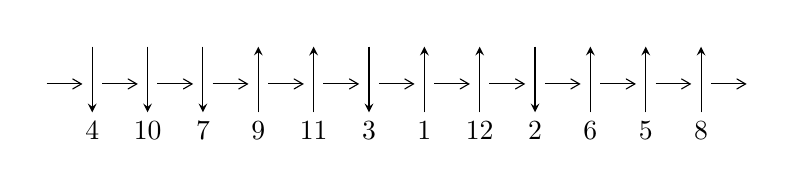
\begin{tikzpicture}[x=20pt, y=17pt]
	% nodes
	\node (C0) at (0, 0) {};
	\node (C1) at (1, 0) {};
	\node (C1U) at (1, +1) {};
	\node (C1D) at (1, -1) {4};

	\node (C2) at (2, 0) {};
	\node (C2U) at (2, +1) {};
	\node (C2D) at (2, -1) {10};

	\node (C3) at (3, 0) {};
	\node (C3U) at (3, +1) {};
	\node (C3D) at (3, -1) {7};

	\node (C4) at (4, 0) {};
	\node (C4U) at (4, +1) {};
	\node (C4D) at (4, -1) {9};

	\node (C5) at (5, 0) {};
	\node (C5U) at (5, +1) {};
	\node (C5D) at (5, -1) {11};

	\node (C6) at (6, 0) {};
	\node (C6U) at (6, +1) {};
	\node (C6D) at (6, -1) {3};

	\node (C7) at (7, 0) {};
	\node (C7U) at (7, +1) {};
	\node (C7D) at (7, -1) {1};

	\node (C8) at (8, 0) {};
	\node (C8U) at (8, +1) {};
	\node (C8D) at (8, -1) {12};

	\node (C9) at (9, 0) {};
	\node (C9U) at (9, +1) {};
	\node (C9D) at (9, -1) {2};

	\node (C10) at (10, 0) {};
	\node (C10U) at (10, +1) {};
	\node (C10D) at (10, -1) {6};

	\node (C11) at (11, 0) {};
	\node (C11U) at (11, +1) {};
	\node (C11D) at (11, -1) {5};

	\node (C12) at (12, 0) {};
	\node (C12U) at (12, +1) {};
	\node (C12D) at (12, -1) {8};
	\node (C13) at (13, 0) {};

	% arrows
	\draw[->,>={angle 60}]
	(C0) edge (C1) (C1) edge (C2) (C2) edge (C3) (C3) edge (C4) (C4) edge (C5) (C5) edge (C6) (C6) edge (C7) (C7) edge (C8) (C8) edge (C9) (C9) edge (C10) (C10) edge (C11) (C11) edge (C12) (C12) edge (C13) ;	\draw[->,>=stealth]
	(C1U) edge (C1D) (C2U) edge (C2D) (C3U) edge (C3D) (C4D) edge (C4U) (C5D) edge (C5U) (C6U) edge (C6D) (C7D) edge (C7U) (C8D) edge (C8U) (C9U) edge (C9D) (C10D) edge (C10U) (C11D) edge (C11U) (C12D) edge (C12U) ;
	\end{tikzpicture} \\
\hhline{~~} \\& 
\textbf{Solving Sequence} \\ \cline{2-2} 
 &
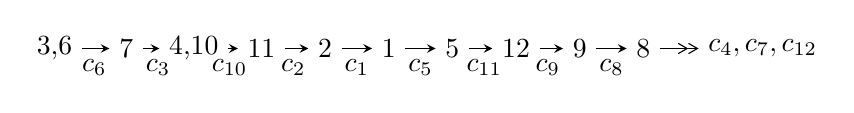
\begin{tikzpicture}[x=23pt, y=7pt]
	% node
	\node (A0) at (-1/8, 0) {3,6};
	\node (A1) at (1, 0) {7};
	\node (A2) at (33/16, 0) {4,10};
	\node (A3) at (25/8, 0) {11};
	\node (A4) at (33/8, 0) {2};
	\node (A5) at (41/8, 0) {1};
	\node (A6) at (49/8, 0) {5};
	\node (A7) at (57/8, 0) {12};
	\node (A8) at (65/8, 0) {9};
	\node (A9) at (73/8, 0) {8};
	\node (C1) at (1/2, -1) {$c_{6}$};
	\node (C2) at (3/2, -1) {$c_{3}$};
	\node (C3) at (21/8, -1) {$c_{10}$};
	\node (C4) at (29/8, -1) {$c_{2}$};
	\node (C5) at (37/8, -1) {$c_{1}$};
	\node (C6) at (45/8, -1) {$c_{5}$};
	\node (C7) at (53/8, -1) {$c_{11}$};
	\node (C8) at (61/8, -1) {$c_{9}$};
	\node (C9) at (69/8, -1) {$c_{8}$};
	\node (A10) at (11, 0) {$c_{4},c_{7},c_{12}$};

	% edge
	\draw[->,>=stealth]	
	(A0) edge (A1) (A1) edge (A2) (A2) edge (A3) (A3) edge (A4) (A4) edge (A5) (A5) edge (A6) (A6) edge (A7) (A7) edge (A8) (A8) edge (A9) ;
	\draw[->>,>={angle 60}]	
	(A9) edge (A10);
\end{tikzpicture} \\ 

\end{tabular} \\

\footnotetext{
The image of knot diagram is generated by the software ``\textbf{Draw programme}" developed by Andrew Bartholomew(\url{http://www.layer8.co.uk/maths/draw/index.htm\#Running-draw}), where we modified some parts for our purpose(\url{https://github.com/CATsTAILs/LinksPainter}).
}\phantom \\ \newline 
\centering \textbf{Ideals for irreducible components\footnotemark of $X_{\text{par}}$} 
 
\begin{align*}
I^u_{1}&=\langle 
1.19554\times10^{254} u^{79}-4.06335\times10^{253} u^{78}+\cdots+6.78866\times10^{255} b-1.22944\times10^{255},\\
\phantom{I^u_{1}}&\phantom{= \langle  }-1.22177\times10^{256} u^{79}+3.50873\times10^{254} u^{78}+\cdots+4.95572\times10^{257} a-3.21558\times10^{258},\\
\phantom{I^u_{1}}&\phantom{= \langle  }u^{80}-42 u^{78}+\cdots+695 u+73\rangle \\
I^u_{2}&=\langle 
-8933 u^{22}+72416 u^{21}+\cdots+26063 b-18756,\\
\phantom{I^u_{2}}&\phantom{= \langle  }-325452679 u^{22}+1996854611 u^{21}+\cdots+187627537 a-428118748,\;u^{23}-5 u^{22}+\cdots-2 u+1\rangle \\
\\
\end{align*}
\raggedright * 2 irreducible components of $\dim_{\mathbb{C}}=0$, with total 103 representations.\\
\footnotetext{All coefficients of polynomials are rational numbers. But the coefficients are sometimes approximated in decimal forms when there is not enough margin.}
\newpage
\renewcommand{\arraystretch}{1}
\centering \section*{I. $I^u_{1}= \langle 1.20\times10^{254} u^{79}-4.06\times10^{253} u^{78}+\cdots+6.79\times10^{255} b-1.23\times10^{255},\;-1.22\times10^{256} u^{79}+3.51\times10^{254} u^{78}+\cdots+4.96\times10^{257} a-3.22\times10^{258},\;u^{80}-42 u^{78}+\cdots+695 u+73 \rangle$}
\flushleft \textbf{(i) Arc colorings}\\
\begin{tabular}{m{7pt} m{180pt} m{7pt} m{180pt} }
\flushright $a_{3}=$&$\begin{pmatrix}0\\u\end{pmatrix}$ \\
\flushright $a_{6}=$&$\begin{pmatrix}1\\0\end{pmatrix}$ \\
\flushright $a_{7}=$&$\begin{pmatrix}1\\u^2\end{pmatrix}$ \\
\flushright $a_{4}=$&$\begin{pmatrix}- u\\- u^3+u\end{pmatrix}$ \\
\flushright $a_{10}=$&$\begin{pmatrix}0.0246538 u^{79}-0.000708015 u^{78}+\cdots+10.2302 u+6.48862\\-0.0176108 u^{79}+0.00598549 u^{78}+\cdots-8.43907 u+0.181103\end{pmatrix}$ \\
\flushright $a_{11}=$&$\begin{pmatrix}0.00704298 u^{79}+0.00527747 u^{78}+\cdots+1.79116 u+6.66973\\-0.0176108 u^{79}+0.00598549 u^{78}+\cdots-8.43907 u+0.181103\end{pmatrix}$ \\
\flushright $a_{2}=$&$\begin{pmatrix}-0.0318869 u^{79}+0.00250679 u^{78}+\cdots+10.8269 u-5.17085\\0.0182869 u^{79}-0.00815417 u^{78}+\cdots+21.5937 u+1.26735\end{pmatrix}$ \\
\flushright $a_{1}=$&$\begin{pmatrix}-0.0126502 u^{79}-0.0195104 u^{78}+\cdots+18.8202 u-4.43663\\0.0286845 u^{79}-0.0261087 u^{78}+\cdots+27.4980 u+2.14039\end{pmatrix}$ \\
\flushright $a_{5}=$&$\begin{pmatrix}0.0000878937 u^{79}+0.000822250 u^{78}+\cdots+46.4529 u+8.89458\\0.0174489 u^{79}-0.0174646 u^{78}+\cdots-1.86747 u-0.633244\end{pmatrix}$ \\
\flushright $a_{12}=$&$\begin{pmatrix}-0.0321181 u^{79}+0.0194870 u^{78}+\cdots+11.6089 u+8.55274\\-0.00592250 u^{79}+0.0298193 u^{78}+\cdots+1.11590 u-0.766760\end{pmatrix}$ \\
\flushright $a_{9}=$&$\begin{pmatrix}-0.00731128 u^{79}+0.00275510 u^{78}+\cdots+52.6202 u+4.29409\\0.00670229 u^{79}-0.00572929 u^{78}+\cdots+1.06723 u+0.396634\end{pmatrix}$ \\
\flushright $a_{8}=$&$\begin{pmatrix}-0.00733362 u^{79}-0.0104153 u^{78}+\cdots-55.9268 u-4.94251\\-0.00542082 u^{79}+0.00217554 u^{78}+\cdots+32.0132 u+3.53866\end{pmatrix}$\\&\end{tabular}
\flushleft \textbf{(ii) Obstruction class $= -1$}\\~\\
\flushleft \textbf{(iii) Cusp Shapes $= 0.0629654 u^{79}-0.0984874 u^{78}+\cdots-37.1337 u-2.30507$}\\~\\
\newpage\renewcommand{\arraystretch}{1}
\flushleft \textbf{(iv) u-Polynomials at the component}\newline \\
\begin{tabular}{m{50pt}|m{274pt}}
Crossings & \hspace{64pt}u-Polynomials at each crossing \\
\hline $$\begin{aligned}c_{1}\end{aligned}$$&$\begin{aligned}
&u^{80}-11 u^{79}+\cdots-1319100 u+193025
\end{aligned}$\\
\hline $$\begin{aligned}c_{2},c_{9}\end{aligned}$$&$\begin{aligned}
&u^{80}- u^{79}+\cdots+37 u+1
\end{aligned}$\\
\hline $$\begin{aligned}c_{3},c_{6}\end{aligned}$$&$\begin{aligned}
&u^{80}-42 u^{78}+\cdots+695 u+73
\end{aligned}$\\
\hline $$\begin{aligned}c_{4}\end{aligned}$$&$\begin{aligned}
&u^{80}+3 u^{79}+\cdots+9720133 u+1148717
\end{aligned}$\\
\hline $$\begin{aligned}c_{5},c_{10},c_{11}\end{aligned}$$&$\begin{aligned}
&u^{80}+u^{79}+\cdots+1161 u+173
\end{aligned}$\\
\hline $$\begin{aligned}c_{7},c_{8},c_{12}\end{aligned}$$&$\begin{aligned}
&u^{80}-2 u^{79}+\cdots+27 u+19
\end{aligned}$\\
\hline
\end{tabular}\\~\\
\newpage\renewcommand{\arraystretch}{1}
\flushleft \textbf{(v) Riley Polynomials at the component}\newline \\
\begin{tabular}{m{50pt}|m{274pt}}
Crossings & \hspace{64pt}Riley Polynomials at each crossing \\
\hline $$\begin{aligned}c_{1}\end{aligned}$$&$\begin{aligned}
&y^{80}-45 y^{79}+\cdots-611400686100 y+37258650625
\end{aligned}$\\
\hline $$\begin{aligned}c_{2},c_{9}\end{aligned}$$&$\begin{aligned}
&y^{80}-69 y^{79}+\cdots+21 y+1
\end{aligned}$\\
\hline $$\begin{aligned}c_{3},c_{6}\end{aligned}$$&$\begin{aligned}
&y^{80}-84 y^{79}+\cdots+146819 y+5329
\end{aligned}$\\
\hline $$\begin{aligned}c_{4}\end{aligned}$$&$\begin{aligned}
&y^{80}+51 y^{79}+\cdots+26316054060919 y+1319550746089
\end{aligned}$\\
\hline $$\begin{aligned}c_{5},c_{10},c_{11}\end{aligned}$$&$\begin{aligned}
&y^{80}+95 y^{79}+\cdots+207349 y+29929
\end{aligned}$\\
\hline $$\begin{aligned}c_{7},c_{8},c_{12}\end{aligned}$$&$\begin{aligned}
&y^{80}+90 y^{79}+\cdots+11507 y+361
\end{aligned}$\\
\hline
\end{tabular}\\~\\
\newpage\flushleft \textbf{(vi) Complex Volumes and Cusp Shapes}
$$\begin{array}{c|c|c}  
\text{Solutions to }I^u_{1}& \I (\text{vol} + \sqrt{-1}CS) & \text{Cusp shape}\\
 \hline 
\begin{aligned}
u &= -0.933025 + 0.257843 I \\
a &= \phantom{-}0.0297219 + 0.0412596 I \\
b &= \phantom{-}0.279840 - 0.440086 I\end{aligned}
 & -1.57667 + 1.00823 I & \phantom{-0.000000 } 0 \\ \hline\begin{aligned}
u &= -0.933025 - 0.257843 I \\
a &= \phantom{-}0.0297219 - 0.0412596 I \\
b &= \phantom{-}0.279840 + 0.440086 I\end{aligned}
 & -1.57667 - 1.00823 I & \phantom{-0.000000 } 0 \\ \hline\begin{aligned}
u &= -0.899699 + 0.132536 I \\
a &= -1.049370 + 0.742428 I \\
b &= -0.022659 + 1.203980 I\end{aligned}
 & -4.83425 + 2.94657 I & \phantom{-0.000000 } 0 \\ \hline\begin{aligned}
u &= -0.899699 - 0.132536 I \\
a &= -1.049370 - 0.742428 I \\
b &= -0.022659 - 1.203980 I\end{aligned}
 & -4.83425 - 2.94657 I & \phantom{-0.000000 } 0 \\ \hline\begin{aligned}
u &= \phantom{-}1.110620 + 0.130479 I \\
a &= -0.231583 - 0.901934 I \\
b &= \phantom{-}0.181838 - 0.539644 I\end{aligned}
 & -1.72864 - 2.75147 I & \phantom{-0.000000 } 0 \\ \hline\begin{aligned}
u &= \phantom{-}1.110620 - 0.130479 I \\
a &= -0.231583 + 0.901934 I \\
b &= \phantom{-}0.181838 + 0.539644 I\end{aligned}
 & -1.72864 + 2.75147 I & \phantom{-0.000000 } 0 \\ \hline\begin{aligned}
u &= \phantom{-}0.156021 + 0.835387 I \\
a &= \phantom{-}0.54574 - 1.58978 I \\
b &= \phantom{-}0.03618 + 1.58404 I\end{aligned}
 & -8.84658 - 0.73985 I & -4.45300 + 0. I\phantom{ +0.000000I} \\ \hline\begin{aligned}
u &= \phantom{-}0.156021 - 0.835387 I \\
a &= \phantom{-}0.54574 + 1.58978 I \\
b &= \phantom{-}0.03618 - 1.58404 I\end{aligned}
 & -8.84658 + 0.73985 I & -4.45300 + 0. I\phantom{ +0.000000I} \\ \hline\begin{aligned}
u &= -0.238929 + 0.796640 I \\
a &= -0.710211 - 1.099990 I \\
b &= \phantom{-}0.317628 + 0.536262 I\end{aligned}
 & -1.58821 + 3.69119 I & \phantom{-0.000000 } 0. - 9.71616 I \\ \hline\begin{aligned}
u &= -0.238929 - 0.796640 I \\
a &= -0.710211 + 1.099990 I \\
b &= \phantom{-}0.317628 - 0.536262 I\end{aligned}
 & -1.58821 - 3.69119 I & \phantom{-0.000000 -}0. + 9.71616 I\\
 \hline 
 \end{array}$$\newpage$$\begin{array}{c|c|c}  
\text{Solutions to }I^u_{1}& \I (\text{vol} + \sqrt{-1}CS) & \text{Cusp shape}\\
 \hline 
\begin{aligned}
u &= -0.107313 + 0.798256 I \\
a &= -0.757440 + 0.103976 I \\
b &= \phantom{-}0.647442 + 0.471902 I\end{aligned}
 & -4.82509 + 2.15434 I & \phantom{-0.000000 } 0. - 3.25418 I \\ \hline\begin{aligned}
u &= -0.107313 - 0.798256 I \\
a &= -0.757440 - 0.103976 I \\
b &= \phantom{-}0.647442 - 0.471902 I\end{aligned}
 & -4.82509 - 2.15434 I & \phantom{-0.000000 -}0. + 3.25418 I \\ \hline\begin{aligned}
u &= -0.377538 + 1.138370 I \\
a &= \phantom{-}0.530912 + 0.824510 I \\
b &= -0.532890 - 0.584575 I\end{aligned}
 & -8.15329 + 5.47182 I & \phantom{-0.000000 } 0 \\ \hline\begin{aligned}
u &= -0.377538 - 1.138370 I \\
a &= \phantom{-}0.530912 - 0.824510 I \\
b &= -0.532890 + 0.584575 I\end{aligned}
 & -8.15329 - 5.47182 I & \phantom{-0.000000 } 0 \\ \hline\begin{aligned}
u &= \phantom{-}0.296833 + 0.728763 I \\
a &= -0.627261 - 0.274114 I \\
b &= \phantom{-}0.22622 - 1.47408 I\end{aligned}
 & -11.11080 - 5.32394 I & -1.60578 + 2.44564 I \\ \hline\begin{aligned}
u &= \phantom{-}0.296833 - 0.728763 I \\
a &= -0.627261 + 0.274114 I \\
b &= \phantom{-}0.22622 + 1.47408 I\end{aligned}
 & -11.11080 + 5.32394 I & -1.60578 - 2.44564 I \\ \hline\begin{aligned}
u &= -0.596798 + 0.368285 I \\
a &= -0.737061 - 1.015400 I \\
b &= \phantom{-}0.147050 + 1.051450 I\end{aligned}
 & -3.90294 - 0.95979 I & -6.90709 - 1.74186 I \\ \hline\begin{aligned}
u &= -0.596798 - 0.368285 I \\
a &= -0.737061 + 1.015400 I \\
b &= \phantom{-}0.147050 - 1.051450 I\end{aligned}
 & -3.90294 + 0.95979 I & -6.90709 + 1.74186 I \\ \hline\begin{aligned}
u &= -1.222420 + 0.458831 I \\
a &= \phantom{-}0.0443970 - 0.0548076 I \\
b &= -0.632083 + 0.462534 I\end{aligned}
 & -8.11023 + 2.43176 I & \phantom{-0.000000 } 0 \\ \hline\begin{aligned}
u &= -1.222420 - 0.458831 I \\
a &= \phantom{-}0.0443970 + 0.0548076 I \\
b &= -0.632083 - 0.462534 I\end{aligned}
 & -8.11023 - 2.43176 I & \phantom{-0.000000 } 0\\
 \hline 
 \end{array}$$\newpage$$\begin{array}{c|c|c}  
\text{Solutions to }I^u_{1}& \I (\text{vol} + \sqrt{-1}CS) & \text{Cusp shape}\\
 \hline 
\begin{aligned}
u &= \phantom{-}1.279500 + 0.360515 I \\
a &= \phantom{-}0.291837 + 0.607605 I \\
b &= -0.474926 + 0.715944 I\end{aligned}
 & -9.11742 - 6.23645 I & \phantom{-0.000000 } 0 \\ \hline\begin{aligned}
u &= \phantom{-}1.279500 - 0.360515 I \\
a &= \phantom{-}0.291837 - 0.607605 I \\
b &= -0.474926 - 0.715944 I\end{aligned}
 & -9.11742 + 6.23645 I & \phantom{-0.000000 } 0 \\ \hline\begin{aligned}
u &= -0.538435 + 0.378124 I \\
a &= \phantom{-}1.121120 + 0.169264 I \\
b &= -0.098631 - 0.827664 I\end{aligned}
 & -0.95937 + 1.55975 I & \phantom{-}2.01700 - 4.77080 I \\ \hline\begin{aligned}
u &= -0.538435 - 0.378124 I \\
a &= \phantom{-}1.121120 - 0.169264 I \\
b &= -0.098631 + 0.827664 I\end{aligned}
 & -0.95937 - 1.55975 I & \phantom{-}2.01700 + 4.77080 I \\ \hline\begin{aligned}
u &= \phantom{-}0.389677 + 1.292350 I \\
a &= -0.431269 + 0.939915 I \\
b &= \phantom{-}0.07554 - 1.56927 I\end{aligned}
 & -8.80812 - 5.04260 I & \phantom{-0.000000 } 0 \\ \hline\begin{aligned}
u &= \phantom{-}0.389677 - 1.292350 I \\
a &= -0.431269 - 0.939915 I \\
b &= \phantom{-}0.07554 + 1.56927 I\end{aligned}
 & -8.80812 + 5.04260 I & \phantom{-0.000000 } 0 \\ \hline\begin{aligned}
u &= -1.360730 + 0.003685 I \\
a &= \phantom{-}0.981515 + 0.029454 I \\
b &= -1.030470 - 0.448078 I\end{aligned}
 & -5.79631 - 1.42222 I & \phantom{-0.000000 } 0 \\ \hline\begin{aligned}
u &= -1.360730 - 0.003685 I \\
a &= \phantom{-}0.981515 - 0.029454 I \\
b &= -1.030470 + 0.448078 I\end{aligned}
 & -5.79631 + 1.42222 I & \phantom{-0.000000 } 0 \\ \hline\begin{aligned}
u &= \phantom{-}1.380500 + 0.156477 I \\
a &= \phantom{-}0.028479 + 0.503486 I \\
b &= \phantom{-}0.07032 + 1.53121 I\end{aligned}
 & -8.24917 + 0.23612 I & \phantom{-0.000000 } 0 \\ \hline\begin{aligned}
u &= \phantom{-}1.380500 - 0.156477 I \\
a &= \phantom{-}0.028479 - 0.503486 I \\
b &= \phantom{-}0.07032 - 1.53121 I\end{aligned}
 & -8.24917 - 0.23612 I & \phantom{-0.000000 } 0\\
 \hline 
 \end{array}$$\newpage$$\begin{array}{c|c|c}  
\text{Solutions to }I^u_{1}& \I (\text{vol} + \sqrt{-1}CS) & \text{Cusp shape}\\
 \hline 
\begin{aligned}
u &= \phantom{-}1.387760 + 0.076721 I \\
a &= -1.053390 - 0.203653 I \\
b &= \phantom{-}0.491717 - 0.666089 I\end{aligned}
 & -6.41963 - 2.52717 I & \phantom{-0.000000 } 0 \\ \hline\begin{aligned}
u &= \phantom{-}1.387760 - 0.076721 I \\
a &= -1.053390 + 0.203653 I \\
b &= \phantom{-}0.491717 + 0.666089 I\end{aligned}
 & -6.41963 + 2.52717 I & \phantom{-0.000000 } 0 \\ \hline\begin{aligned}
u &= \phantom{-}1.389780 + 0.140595 I \\
a &= -1.021750 - 0.096001 I \\
b &= \phantom{-}0.44598 - 1.81464 I\end{aligned}
 & \phantom{-}19.1249 - 4.0847 I & \phantom{-0.000000 } 0 \\ \hline\begin{aligned}
u &= \phantom{-}1.389780 - 0.140595 I \\
a &= -1.021750 + 0.096001 I \\
b &= \phantom{-}0.44598 + 1.81464 I\end{aligned}
 & \phantom{-}19.1249 + 4.0847 I & \phantom{-0.000000 } 0 \\ \hline\begin{aligned}
u &= -1.395520 + 0.114360 I \\
a &= -0.974540 - 0.048957 I \\
b &= \phantom{-}1.35472 - 0.51672 I\end{aligned}
 & -12.74490 + 2.98456 I & \phantom{-0.000000 } 0 \\ \hline\begin{aligned}
u &= -1.395520 - 0.114360 I \\
a &= -0.974540 + 0.048957 I \\
b &= \phantom{-}1.35472 + 0.51672 I\end{aligned}
 & -12.74490 - 2.98456 I & \phantom{-0.000000 } 0 \\ \hline\begin{aligned}
u &= -1.42165 + 0.06964 I \\
a &= -0.156336 + 1.118770 I \\
b &= \phantom{-}0.04076 + 1.58926 I\end{aligned}
 & -9.17850 + 3.49089 I & \phantom{-0.000000 } 0 \\ \hline\begin{aligned}
u &= -1.42165 - 0.06964 I \\
a &= -0.156336 - 1.118770 I \\
b &= \phantom{-}0.04076 - 1.58926 I\end{aligned}
 & -9.17850 - 3.49089 I & \phantom{-0.000000 } 0 \\ \hline\begin{aligned}
u &= \phantom{-}0.568595 + 0.041815 I \\
a &= -1.24087 - 1.09976 I \\
b &= \phantom{-}0.251287 - 0.048586 I\end{aligned}
 & -0.93338 - 2.24071 I & \phantom{-}7.29920 + 5.10530 I \\ \hline\begin{aligned}
u &= \phantom{-}0.568595 - 0.041815 I \\
a &= -1.24087 + 1.09976 I \\
b &= \phantom{-}0.251287 + 0.048586 I\end{aligned}
 & -0.93338 + 2.24071 I & \phantom{-}7.29920 - 5.10530 I\\
 \hline 
 \end{array}$$\newpage$$\begin{array}{c|c|c}  
\text{Solutions to }I^u_{1}& \I (\text{vol} + \sqrt{-1}CS) & \text{Cusp shape}\\
 \hline 
\begin{aligned}
u &= \phantom{-}1.42349 + 0.25160 I \\
a &= \phantom{-}1.010970 + 0.049425 I \\
b &= -0.768916 + 0.774349 I\end{aligned}
 & -6.98740 - 7.32316 I & \phantom{-0.000000 } 0 \\ \hline\begin{aligned}
u &= \phantom{-}1.42349 - 0.25160 I \\
a &= \phantom{-}1.010970 - 0.049425 I \\
b &= -0.768916 - 0.774349 I\end{aligned}
 & -6.98740 + 7.32316 I & \phantom{-0.000000 } 0 \\ \hline\begin{aligned}
u &= \phantom{-}1.40704 + 0.36853 I \\
a &= \phantom{-}0.969961 - 0.058572 I \\
b &= -0.31592 + 1.66165 I\end{aligned}
 & -12.91650 - 3.79429 I & \phantom{-0.000000 } 0 \\ \hline\begin{aligned}
u &= \phantom{-}1.40704 - 0.36853 I \\
a &= \phantom{-}0.969961 + 0.058572 I \\
b &= -0.31592 - 1.66165 I\end{aligned}
 & -12.91650 + 3.79429 I & \phantom{-0.000000 } 0 \\ \hline\begin{aligned}
u &= -1.45273 + 0.14202 I \\
a &= \phantom{-}1.122970 - 0.440056 I \\
b &= -0.04410 - 1.63069 I\end{aligned}
 & \phantom{-}18.3007 - 0.5410 I & \phantom{-0.000000 } 0 \\ \hline\begin{aligned}
u &= -1.45273 - 0.14202 I \\
a &= \phantom{-}1.122970 + 0.440056 I \\
b &= -0.04410 + 1.63069 I\end{aligned}
 & \phantom{-}18.3007 + 0.5410 I & \phantom{-0.000000 } 0 \\ \hline\begin{aligned}
u &= -1.46987 + 0.27140 I \\
a &= -0.851510 - 0.167573 I \\
b &= \phantom{-}0.509179 + 0.438607 I\end{aligned}
 & -5.64665 + 1.00939 I & \phantom{-0.000000 } 0 \\ \hline\begin{aligned}
u &= -1.46987 - 0.27140 I \\
a &= -0.851510 + 0.167573 I \\
b &= \phantom{-}0.509179 - 0.438607 I\end{aligned}
 & -5.64665 - 1.00939 I & \phantom{-0.000000 } 0 \\ \hline\begin{aligned}
u &= -1.46286 + 0.30961 I \\
a &= -1.193090 + 0.207085 I \\
b &= \phantom{-}0.14007 + 1.61352 I\end{aligned}
 & -14.2338 + 4.8692 I & \phantom{-0.000000 } 0 \\ \hline\begin{aligned}
u &= -1.46286 - 0.30961 I \\
a &= -1.193090 - 0.207085 I \\
b &= \phantom{-}0.14007 - 1.61352 I\end{aligned}
 & -14.2338 - 4.8692 I & \phantom{-0.000000 } 0\\
 \hline 
 \end{array}$$\newpage$$\begin{array}{c|c|c}  
\text{Solutions to }I^u_{1}& \I (\text{vol} + \sqrt{-1}CS) & \text{Cusp shape}\\
 \hline 
\begin{aligned}
u &= \phantom{-}1.49177 + 0.17819 I \\
a &= \phantom{-}0.880021 - 0.391812 I \\
b &= -0.145201 - 0.700742 I\end{aligned}
 & -12.98350 - 1.27674 I & \phantom{-0.000000 } 0 \\ \hline\begin{aligned}
u &= \phantom{-}1.49177 - 0.17819 I \\
a &= \phantom{-}0.880021 + 0.391812 I \\
b &= -0.145201 + 0.700742 I\end{aligned}
 & -12.98350 + 1.27674 I & \phantom{-0.000000 } 0 \\ \hline\begin{aligned}
u &= -1.49301 + 0.20563 I \\
a &= \phantom{-}0.271872 - 0.890511 I \\
b &= -0.12925 - 1.62695 I\end{aligned}
 & -17.1793 + 8.4656 I & \phantom{-0.000000 } 0 \\ \hline\begin{aligned}
u &= -1.49301 - 0.20563 I \\
a &= \phantom{-}0.271872 + 0.890511 I \\
b &= -0.12925 + 1.62695 I\end{aligned}
 & -17.1793 - 8.4656 I & \phantom{-0.000000 } 0 \\ \hline\begin{aligned}
u &= \phantom{-}1.50221 + 0.34705 I \\
a &= -0.941368 + 0.004617 I \\
b &= \phantom{-}0.960337 - 0.913714 I\end{aligned}
 & -14.2323 - 10.4782 I & \phantom{-0.000000 } 0 \\ \hline\begin{aligned}
u &= \phantom{-}1.50221 - 0.34705 I \\
a &= -0.941368 - 0.004617 I \\
b &= \phantom{-}0.960337 + 0.913714 I\end{aligned}
 & -14.2323 + 10.4782 I & \phantom{-0.000000 } 0 \\ \hline\begin{aligned}
u &= \phantom{-}0.155519 + 0.409623 I \\
a &= \phantom{-}1.175290 - 0.037639 I \\
b &= -0.427697 - 0.189345 I\end{aligned}
 & \phantom{-}0.861772 + 0.593079 I & \phantom{-}8.14040 - 3.49994 I \\ \hline\begin{aligned}
u &= \phantom{-}0.155519 - 0.409623 I \\
a &= \phantom{-}1.175290 + 0.037639 I \\
b &= -0.427697 + 0.189345 I\end{aligned}
 & \phantom{-}0.861772 - 0.593079 I & \phantom{-}8.14040 + 3.49994 I \\ \hline\begin{aligned}
u &= \phantom{-}1.53473 + 0.32845 I \\
a &= -0.040041 - 0.446319 I \\
b &= -0.15983 - 1.61623 I\end{aligned}
 & -15.4607 + 0.5021 I & \phantom{-0.000000 } 0 \\ \hline\begin{aligned}
u &= \phantom{-}1.53473 - 0.32845 I \\
a &= -0.040041 + 0.446319 I \\
b &= -0.15983 + 1.61623 I\end{aligned}
 & -15.4607 - 0.5021 I & \phantom{-0.000000 } 0\\
 \hline 
 \end{array}$$\newpage$$\begin{array}{c|c|c}  
\text{Solutions to }I^u_{1}& \I (\text{vol} + \sqrt{-1}CS) & \text{Cusp shape}\\
 \hline 
\begin{aligned}
u &= \phantom{-}0.018150 + 0.396081 I \\
a &= \phantom{-}1.04718 - 2.72969 I \\
b &= -0.711168 - 0.566289 I\end{aligned}
 & -7.94238 - 1.27246 I & -5.21046 - 0.09579 I \\ \hline\begin{aligned}
u &= \phantom{-}0.018150 - 0.396081 I \\
a &= \phantom{-}1.04718 + 2.72969 I \\
b &= -0.711168 + 0.566289 I\end{aligned}
 & -7.94238 + 1.27246 I & -5.21046 + 0.09579 I \\ \hline\begin{aligned}
u &= -1.56074 + 0.43665 I \\
a &= \phantom{-}1.059430 - 0.062610 I \\
b &= -0.22521 - 1.64176 I\end{aligned}
 & -15.0846 + 11.0453 I & \phantom{-0.000000 } 0 \\ \hline\begin{aligned}
u &= -1.56074 - 0.43665 I \\
a &= \phantom{-}1.059430 + 0.062610 I \\
b &= -0.22521 + 1.64176 I\end{aligned}
 & -15.0846 - 11.0453 I & \phantom{-0.000000 } 0 \\ \hline\begin{aligned}
u &= \phantom{-}0.080693 + 0.331904 I \\
a &= -1.63830 + 3.85989 I \\
b &= -0.19093 - 1.67778 I\end{aligned}
 & -15.8360 + 2.3469 I & -8.33417 - 0.26186 I \\ \hline\begin{aligned}
u &= \phantom{-}0.080693 - 0.331904 I \\
a &= -1.63830 - 3.85989 I \\
b &= -0.19093 + 1.67778 I\end{aligned}
 & -15.8360 - 2.3469 I & -8.33417 + 0.26186 I \\ \hline\begin{aligned}
u &= \phantom{-}0.095857 + 0.299058 I \\
a &= \phantom{-}1.85934 + 0.46152 I \\
b &= -0.092790 + 1.367820 I\end{aligned}
 & -4.02985 - 2.33762 I & \phantom{-}2.59507 + 2.31518 I \\ \hline\begin{aligned}
u &= \phantom{-}0.095857 - 0.299058 I \\
a &= \phantom{-}1.85934 - 0.46152 I \\
b &= -0.092790 - 1.367820 I\end{aligned}
 & -4.02985 + 2.33762 I & \phantom{-}2.59507 - 2.31518 I \\ \hline\begin{aligned}
u &= -1.68949 + 0.48697 I \\
a &= -0.937193 + 0.047303 I \\
b &= \phantom{-}0.28129 + 1.70007 I\end{aligned}
 & \phantom{-}16.5778 + 15.2060 I & \phantom{-0.000000 } 0 \\ \hline\begin{aligned}
u &= -1.68949 - 0.48697 I \\
a &= -0.937193 - 0.047303 I \\
b &= \phantom{-}0.28129 - 1.70007 I\end{aligned}
 & \phantom{-}16.5778 - 15.2060 I & \phantom{-0.000000 } 0\\
 \hline 
 \end{array}$$\newpage$$\begin{array}{c|c|c}  
\text{Solutions to }I^u_{1}& \I (\text{vol} + \sqrt{-1}CS) & \text{Cusp shape}\\
 \hline 
\begin{aligned}
u &= \phantom{-}0.63666 + 1.69281 I \\
a &= \phantom{-}0.360260 - 0.664641 I \\
b &= -0.14249 + 1.58434 I\end{aligned}
 & -15.5302 - 7.8644 I & \phantom{-0.000000 } 0 \\ \hline\begin{aligned}
u &= \phantom{-}0.63666 - 1.69281 I \\
a &= \phantom{-}0.360260 + 0.664641 I \\
b &= -0.14249 - 1.58434 I\end{aligned}
 & -15.5302 + 7.8644 I & \phantom{-0.000000 } 0 \\ \hline\begin{aligned}
u &= -1.75601 + 0.59770 I \\
a &= \phantom{-}0.662793 + 0.226410 I \\
b &= -0.139860 - 0.490757 I\end{aligned}
 & -12.23370 + 2.28182 I & \phantom{-0.000000 } 0 \\ \hline\begin{aligned}
u &= -1.75601 - 0.59770 I \\
a &= \phantom{-}0.662793 - 0.226410 I \\
b &= -0.139860 + 0.490757 I\end{aligned}
 & -12.23370 - 2.28182 I & \phantom{-0.000000 } 0 \\ \hline\begin{aligned}
u &= \phantom{-}1.71422 + 0.74113 I \\
a &= -0.718767 + 0.152487 I \\
b &= \phantom{-}0.13592 - 1.55702 I\end{aligned}
 & -12.48250 - 3.26508 I & \phantom{-0.000000 } 0 \\ \hline\begin{aligned}
u &= \phantom{-}1.71422 - 0.74113 I \\
a &= -0.718767 - 0.152487 I \\
b &= \phantom{-}0.13592 + 1.55702 I\end{aligned}
 & -12.48250 + 3.26508 I & \phantom{-0.000000 } 0 \\ \hline\begin{aligned}
u &= -0.0918845 + 0.0886132 I \\
a &= \phantom{-}7.50598 + 2.95587 I \\
b &= \phantom{-}0.236793 - 0.529885 I\end{aligned}
 & -1.43444 + 1.51364 I & \phantom{-}0.75693 + 3.72542 I \\ \hline\begin{aligned}
u &= -0.0918845 - 0.0886132 I \\
a &= \phantom{-}7.50598 - 2.95587 I \\
b &= \phantom{-}0.236793 + 0.529885 I\end{aligned}
 & -1.43444 - 1.51364 I & \phantom{-}0.75693 - 3.72542 I \\ \hline\begin{aligned}
u &= \phantom{-}2.04902 + 0.91722 I \\
a &= \phantom{-}0.585507 - 0.130441 I \\
b &= -0.04510 + 1.57018 I\end{aligned}
 & -19.4247 - 2.9683 I & \phantom{-0.000000 } 0 \\ \hline\begin{aligned}
u &= \phantom{-}2.04902 - 0.91722 I \\
a &= \phantom{-}0.585507 + 0.130441 I \\
b &= -0.04510 - 1.57018 I\end{aligned}
 & -19.4247 + 2.9683 I & \phantom{-0.000000 } 0\\
 \hline 
 \end{array}$$\newpage\newpage\renewcommand{\arraystretch}{1}
\centering \section*{II. $I^u_{2}= \langle -8933 u^{22}+72416 u^{21}+\cdots+26063 b-18756,\;-3.25\times10^{8} u^{22}+2.00\times10^{9} u^{21}+\cdots+1.88\times10^{8} a-4.28\times10^{8},\;u^{23}-5 u^{22}+\cdots-2 u+1 \rangle$}
\flushleft \textbf{(i) Arc colorings}\\
\begin{tabular}{m{7pt} m{180pt} m{7pt} m{180pt} }
\flushright $a_{3}=$&$\begin{pmatrix}0\\u\end{pmatrix}$ \\
\flushright $a_{6}=$&$\begin{pmatrix}1\\0\end{pmatrix}$ \\
\flushright $a_{7}=$&$\begin{pmatrix}1\\u^2\end{pmatrix}$ \\
\flushright $a_{4}=$&$\begin{pmatrix}- u\\- u^3+u\end{pmatrix}$ \\
\flushright $a_{10}=$&$\begin{pmatrix}1.73457 u^{22}-10.6427 u^{21}+\cdots+15.7223 u+2.28175\\0.342746 u^{22}-2.77850 u^{21}+\cdots-6.43487 u+0.719641\end{pmatrix}$ \\
\flushright $a_{11}=$&$\begin{pmatrix}2.07731 u^{22}-13.4212 u^{21}+\cdots+9.28739 u+3.00139\\0.342746 u^{22}-2.77850 u^{21}+\cdots-6.43487 u+0.719641\end{pmatrix}$ \\
\flushright $a_{2}=$&$\begin{pmatrix}1.56835 u^{22}-8.77970 u^{21}+\cdots-21.4092 u-1.02035\\0.844437 u^{22}-3.99394 u^{21}+\cdots+4.08247 u+0.437912\end{pmatrix}$ \\
\flushright $a_{1}=$&$\begin{pmatrix}2.32346 u^{22}-12.7898 u^{21}+\cdots-22.9240 u-0.404159\\0.773141 u^{22}-3.43217 u^{21}+\cdots+4.37302 u+0.0562597\end{pmatrix}$ \\
\flushright $a_{5}=$&$\begin{pmatrix}-0.437912 u^{22}+3.03400 u^{21}+\cdots-4.03499 u+3.95829\\- u-1\end{pmatrix}$ \\
\flushright $a_{12}=$&$\begin{pmatrix}3.37733 u^{22}-17.7045 u^{21}+\cdots-13.5909 u+2.79696\\1.06477 u^{22}-4.72597 u^{21}+\cdots-1.40513 u+0.342746\end{pmatrix}$ \\
\flushright $a_{9}=$&$\begin{pmatrix}0.757435 u^{22}-5.67549 u^{21}+\cdots+11.9765 u-2.55321\\-0.344110 u^{22}+1.85506 u^{21}+\cdots+1.66476 u-0.242129\end{pmatrix}$ \\
\flushright $a_{8}=$&$\begin{pmatrix}0.904547 u^{22}-5.79853 u^{21}+\cdots+16.1850 u-1.78107\\-0.595303 u^{22}+3.54364 u^{21}+\cdots+1.40322 u-0.225478\end{pmatrix}$\\&\end{tabular}
\flushleft \textbf{(ii) Obstruction class $= 1$}\\~\\
\flushleft \textbf{(iii) Cusp Shapes $= \frac{516876394}{187627537} u^{22}-\frac{2115207184}{187627537} u^{21}+\cdots-\frac{1488236262}{187627537} u-\frac{1412792583}{187627537}$}\\~\\
\newpage\renewcommand{\arraystretch}{1}
\flushleft \textbf{(iv) u-Polynomials at the component}\newline \\
\begin{tabular}{m{50pt}|m{274pt}}
Crossings & \hspace{64pt}u-Polynomials at each crossing \\
\hline $$\begin{aligned}c_{1}\end{aligned}$$&$\begin{aligned}
&u^{23}-4 u^{22}+\cdots-7 u+1
\end{aligned}$\\
\hline $$\begin{aligned}c_{2}\end{aligned}$$&$\begin{aligned}
&u^{23}-8 u^{21}+\cdots-5 u^2+1
\end{aligned}$\\
\hline $$\begin{aligned}c_{3}\end{aligned}$$&$\begin{aligned}
&u^{23}+5 u^{22}+\cdots-2 u-1
\end{aligned}$\\
\hline $$\begin{aligned}c_{4}\end{aligned}$$&$\begin{aligned}
&u^{23}+4 u^{21}+\cdots-6 u-1
\end{aligned}$\\
\hline $$\begin{aligned}c_{5}\end{aligned}$$&$\begin{aligned}
&u^{23}+14 u^{21}+\cdots-13 u^2-1
\end{aligned}$\\
\hline $$\begin{aligned}c_{6}\end{aligned}$$&$\begin{aligned}
&u^{23}-5 u^{22}+\cdots-2 u+1
\end{aligned}$\\
\hline $$\begin{aligned}c_{7},c_{8}\end{aligned}$$&$\begin{aligned}
&u^{23}- u^{22}+\cdots+2 u^2-1
\end{aligned}$\\
\hline $$\begin{aligned}c_{9}\end{aligned}$$&$\begin{aligned}
&u^{23}-8 u^{21}+\cdots+5 u^2-1
\end{aligned}$\\
\hline $$\begin{aligned}c_{10},c_{11}\end{aligned}$$&$\begin{aligned}
&u^{23}+14 u^{21}+\cdots+13 u^2+1
\end{aligned}$\\
\hline $$\begin{aligned}c_{12}\end{aligned}$$&$\begin{aligned}
&u^{23}+u^{22}+\cdots-2 u^2+1
\end{aligned}$\\
\hline
\end{tabular}\\~\\
\newpage\renewcommand{\arraystretch}{1}
\flushleft \textbf{(v) Riley Polynomials at the component}\newline \\
\begin{tabular}{m{50pt}|m{274pt}}
Crossings & \hspace{64pt}Riley Polynomials at each crossing \\
\hline $$\begin{aligned}c_{1}\end{aligned}$$&$\begin{aligned}
&y^{23}-8 y^{22}+\cdots+11 y-1
\end{aligned}$\\
\hline $$\begin{aligned}c_{2},c_{9}\end{aligned}$$&$\begin{aligned}
&y^{23}-16 y^{22}+\cdots+10 y-1
\end{aligned}$\\
\hline $$\begin{aligned}c_{3},c_{6}\end{aligned}$$&$\begin{aligned}
&y^{23}-27 y^{22}+\cdots-36 y-1
\end{aligned}$\\
\hline $$\begin{aligned}c_{4}\end{aligned}$$&$\begin{aligned}
&y^{23}+8 y^{22}+\cdots-32 y-1
\end{aligned}$\\
\hline $$\begin{aligned}c_{5},c_{10},c_{11}\end{aligned}$$&$\begin{aligned}
&y^{23}+28 y^{22}+\cdots-26 y-1
\end{aligned}$\\
\hline $$\begin{aligned}c_{7},c_{8},c_{12}\end{aligned}$$&$\begin{aligned}
&y^{23}+27 y^{22}+\cdots+4 y-1
\end{aligned}$\\
\hline
\end{tabular}\\~\\
\newpage\flushleft \textbf{(vi) Complex Volumes and Cusp Shapes}
$$\begin{array}{c|c|c}  
\text{Solutions to }I^u_{2}& \I (\text{vol} + \sqrt{-1}CS) & \text{Cusp shape}\\
 \hline 
\begin{aligned}
u &= \phantom{-}0.757600 + 0.580515 I \\
a &= \phantom{-}0.593505 - 0.234801 I \\
b &= \phantom{-}0.216088 - 1.343240 I\end{aligned}
 & -12.22340 - 5.69838 I & -9.25274 + 4.18072 I \\ \hline\begin{aligned}
u &= \phantom{-}0.757600 - 0.580515 I \\
a &= \phantom{-}0.593505 + 0.234801 I \\
b &= \phantom{-}0.216088 + 1.343240 I\end{aligned}
 & -12.22340 + 5.69838 I & -9.25274 - 4.18072 I \\ \hline\begin{aligned}
u &= -0.901939 + 0.010790 I \\
a &= -0.578634 + 0.851146 I \\
b &= -0.017203 + 0.313619 I\end{aligned}
 & -1.46016 + 2.03887 I & -5.32019 + 0.28073 I \\ \hline\begin{aligned}
u &= -0.901939 - 0.010790 I \\
a &= -0.578634 - 0.851146 I \\
b &= -0.017203 - 0.313619 I\end{aligned}
 & -1.46016 - 2.03887 I & -5.32019 - 0.28073 I \\ \hline\begin{aligned}
u &= -1.037860 + 0.492778 I \\
a &= \phantom{-}0.707359 + 0.115829 I \\
b &= \phantom{-}0.515794 - 0.477688 I\end{aligned}
 & -8.90749 + 3.00064 I & -9.05512 - 3.71283 I \\ \hline\begin{aligned}
u &= -1.037860 - 0.492778 I \\
a &= \phantom{-}0.707359 - 0.115829 I \\
b &= \phantom{-}0.515794 + 0.477688 I\end{aligned}
 & -8.90749 - 3.00064 I & -9.05512 + 3.71283 I \\ \hline\begin{aligned}
u &= \phantom{-}0.691752 + 0.160792 I \\
a &= -0.536177 - 0.443693 I \\
b &= -0.061742 + 1.302140 I\end{aligned}
 & -4.78747 - 2.56115 I & -8.34774 + 4.70612 I \\ \hline\begin{aligned}
u &= \phantom{-}0.691752 - 0.160792 I \\
a &= -0.536177 + 0.443693 I \\
b &= -0.061742 - 1.302140 I\end{aligned}
 & -4.78747 + 2.56115 I & -8.34774 - 4.70612 I \\ \hline\begin{aligned}
u &= -0.655673 + 0.212810 I \\
a &= -1.321680 + 0.225264 I \\
b &= -0.173862 + 0.612009 I\end{aligned}
 & -1.83707 + 1.99638 I & -8.40872 - 6.71639 I \\ \hline\begin{aligned}
u &= -0.655673 - 0.212810 I \\
a &= -1.321680 - 0.225264 I \\
b &= -0.173862 - 0.612009 I\end{aligned}
 & -1.83707 - 1.99638 I & -8.40872 + 6.71639 I\\
 \hline 
 \end{array}$$\newpage$$\begin{array}{c|c|c}  
\text{Solutions to }I^u_{2}& \I (\text{vol} + \sqrt{-1}CS) & \text{Cusp shape}\\
 \hline 
\begin{aligned}
u &= \phantom{-}1.344240 + 0.025801 I \\
a &= -0.361149 - 0.831706 I \\
b &= \phantom{-}0.00843 - 1.53111 I\end{aligned}
 & -7.95471 - 2.08579 I & -5.56064 + 2.41042 I \\ \hline\begin{aligned}
u &= \phantom{-}1.344240 - 0.025801 I \\
a &= -0.361149 + 0.831706 I \\
b &= \phantom{-}0.00843 + 1.53111 I\end{aligned}
 & -7.95471 + 2.08579 I & -5.56064 - 2.41042 I \\ \hline\begin{aligned}
u &= -1.45736\phantom{ +0.000000I} \\
a &= -0.923005\phantom{ +0.000000I} \\
b &= \phantom{-}0.676281\phantom{ +0.000000I}\end{aligned}
 & -5.64416\phantom{ +0.000000I} & -6.21070\phantom{ +0.000000I} \\ \hline\begin{aligned}
u &= -1.50060 + 0.27712 I \\
a &= \phantom{-}0.805496 + 0.225842 I \\
b &= -0.732389 + 0.189191 I\end{aligned}
 & -10.92140 + 1.50372 I & -5.21005 + 0.05843 I \\ \hline\begin{aligned}
u &= -1.50060 - 0.27712 I \\
a &= \phantom{-}0.805496 - 0.225842 I \\
b &= -0.732389 - 0.189191 I\end{aligned}
 & -10.92140 - 1.50372 I & -5.21005 - 0.05843 I \\ \hline\begin{aligned}
u &= \phantom{-}1.31555 + 0.81648 I \\
a &= \phantom{-}0.810501 - 0.429665 I \\
b &= -0.26432 + 1.54448 I\end{aligned}
 & -16.0466 - 5.3224 I & -9.22028 + 3.35316 I \\ \hline\begin{aligned}
u &= \phantom{-}1.31555 - 0.81648 I \\
a &= \phantom{-}0.810501 + 0.429665 I \\
b &= -0.26432 - 1.54448 I\end{aligned}
 & -16.0466 + 5.3224 I & -9.22028 - 3.35316 I \\ \hline\begin{aligned}
u &= \phantom{-}1.46966 + 0.55634 I \\
a &= -0.904069 + 0.122289 I \\
b &= \phantom{-}0.17591 - 1.58133 I\end{aligned}
 & -11.72400 - 3.23681 I & -1.85835 + 0.78114 I \\ \hline\begin{aligned}
u &= \phantom{-}1.46966 - 0.55634 I \\
a &= -0.904069 - 0.122289 I \\
b &= \phantom{-}0.17591 + 1.58133 I\end{aligned}
 & -11.72400 + 3.23681 I & -1.85835 - 0.78114 I \\ \hline\begin{aligned}
u &= \phantom{-}1.72260 + 0.33154 I \\
a &= \phantom{-}0.681003 + 0.099571 I \\
b &= -0.10028 + 1.65308 I\end{aligned}
 & -18.2680 - 1.7097 I & -8.26819 + 0.20200 I\\
 \hline 
 \end{array}$$\newpage$$\begin{array}{c|c|c}  
\text{Solutions to }I^u_{2}& \I (\text{vol} + \sqrt{-1}CS) & \text{Cusp shape}\\
 \hline 
\begin{aligned}
u &= \phantom{-}1.72260 - 0.33154 I \\
a &= \phantom{-}0.681003 - 0.099571 I \\
b &= -0.10028 - 1.65308 I\end{aligned}
 & -18.2680 + 1.7097 I & -8.26819 - 0.20200 I \\ \hline\begin{aligned}
u &= \phantom{-}0.023342 + 0.193953 I \\
a &= \phantom{-}2.06534 + 5.01376 I \\
b &= \phantom{-}0.095440 - 1.016100 I\end{aligned}
 & -3.38863 + 2.01739 I & -3.39262 - 3.26924 I \\ \hline\begin{aligned}
u &= \phantom{-}0.023342 - 0.193953 I \\
a &= \phantom{-}2.06534 - 5.01376 I \\
b &= \phantom{-}0.095440 + 1.016100 I\end{aligned}
 & -3.38863 - 2.01739 I & -3.39262 + 3.26924 I\\
 \hline 
 \end{array}$$\newpage
\newpage\renewcommand{\arraystretch}{1}
\centering \section*{ III. u-Polynomials}
\begin{tabular}{m{50pt}|m{274pt}}
Crossings & \hspace{64pt}u-Polynomials at each crossing \\
\hline $$\begin{aligned}c_{1}\end{aligned}$$&$\begin{aligned}
&(u^{23}-4 u^{22}+\cdots-7 u+1)(u^{80}-11 u^{79}+\cdots-1319100 u+193025)
\end{aligned}$\\
\hline $$\begin{aligned}c_{2}\end{aligned}$$&$\begin{aligned}
&(u^{23}-8 u^{21}+\cdots-5 u^2+1)(u^{80}- u^{79}+\cdots+37 u+1)
\end{aligned}$\\
\hline $$\begin{aligned}c_{3}\end{aligned}$$&$\begin{aligned}
&(u^{23}+5 u^{22}+\cdots-2 u-1)(u^{80}-42 u^{78}+\cdots+695 u+73)
\end{aligned}$\\
\hline $$\begin{aligned}c_{4}\end{aligned}$$&$\begin{aligned}
&(u^{23}+4 u^{21}+\cdots-6 u-1)(u^{80}+3 u^{79}+\cdots+9720133 u+1148717)
\end{aligned}$\\
\hline $$\begin{aligned}c_{5}\end{aligned}$$&$\begin{aligned}
&(u^{23}+14 u^{21}+\cdots-13 u^2-1)(u^{80}+u^{79}+\cdots+1161 u+173)
\end{aligned}$\\
\hline $$\begin{aligned}c_{6}\end{aligned}$$&$\begin{aligned}
&(u^{23}-5 u^{22}+\cdots-2 u+1)(u^{80}-42 u^{78}+\cdots+695 u+73)
\end{aligned}$\\
\hline $$\begin{aligned}c_{7},c_{8}\end{aligned}$$&$\begin{aligned}
&(u^{23}- u^{22}+\cdots+2 u^2-1)(u^{80}-2 u^{79}+\cdots+27 u+19)
\end{aligned}$\\
\hline $$\begin{aligned}c_{9}\end{aligned}$$&$\begin{aligned}
&(u^{23}-8 u^{21}+\cdots+5 u^2-1)(u^{80}- u^{79}+\cdots+37 u+1)
\end{aligned}$\\
\hline $$\begin{aligned}c_{10},c_{11}\end{aligned}$$&$\begin{aligned}
&(u^{23}+14 u^{21}+\cdots+13 u^2+1)(u^{80}+u^{79}+\cdots+1161 u+173)
\end{aligned}$\\
\hline $$\begin{aligned}c_{12}\end{aligned}$$&$\begin{aligned}
&(u^{23}+u^{22}+\cdots-2 u^2+1)(u^{80}-2 u^{79}+\cdots+27 u+19)
\end{aligned}$\\
\hline
\end{tabular}\newpage\renewcommand{\arraystretch}{1}
\centering \section*{ IV. Riley Polynomials}
\begin{tabular}{m{50pt}|m{274pt}}
Crossings & \hspace{64pt}Riley Polynomials at each crossing \\
\hline $$\begin{aligned}c_{1}\end{aligned}$$&$\begin{aligned}
&(y^{23}-8 y^{22}+\cdots+11 y-1)\\
&\cdot(y^{80}-45 y^{79}+\cdots-611400686100 y+37258650625)
\end{aligned}$\\
\hline $$\begin{aligned}c_{2},c_{9}\end{aligned}$$&$\begin{aligned}
&(y^{23}-16 y^{22}+\cdots+10 y-1)(y^{80}-69 y^{79}+\cdots+21 y+1)
\end{aligned}$\\
\hline $$\begin{aligned}c_{3},c_{6}\end{aligned}$$&$\begin{aligned}
&(y^{23}-27 y^{22}+\cdots-36 y-1)(y^{80}-84 y^{79}+\cdots+146819 y+5329)
\end{aligned}$\\
\hline $$\begin{aligned}c_{4}\end{aligned}$$&$\begin{aligned}
&(y^{23}+8 y^{22}+\cdots-32 y-1)\\
&\cdot(y^{80}+51 y^{79}+\cdots+26316054060919 y+1319550746089)
\end{aligned}$\\
\hline $$\begin{aligned}c_{5},c_{10},c_{11}\end{aligned}$$&$\begin{aligned}
&(y^{23}+28 y^{22}+\cdots-26 y-1)(y^{80}+95 y^{79}+\cdots+207349 y+29929)
\end{aligned}$\\
\hline $$\begin{aligned}c_{7},c_{8},c_{12}\end{aligned}$$&$\begin{aligned}
&(y^{23}+27 y^{22}+\cdots+4 y-1)(y^{80}+90 y^{79}+\cdots+11507 y+361)
\end{aligned}$\\
\hline
\end{tabular}
\vskip 2pc
\end{document}